

\tikzset{every picture/.style={line width=0.3pt}} %set default line width to 0.75pt        

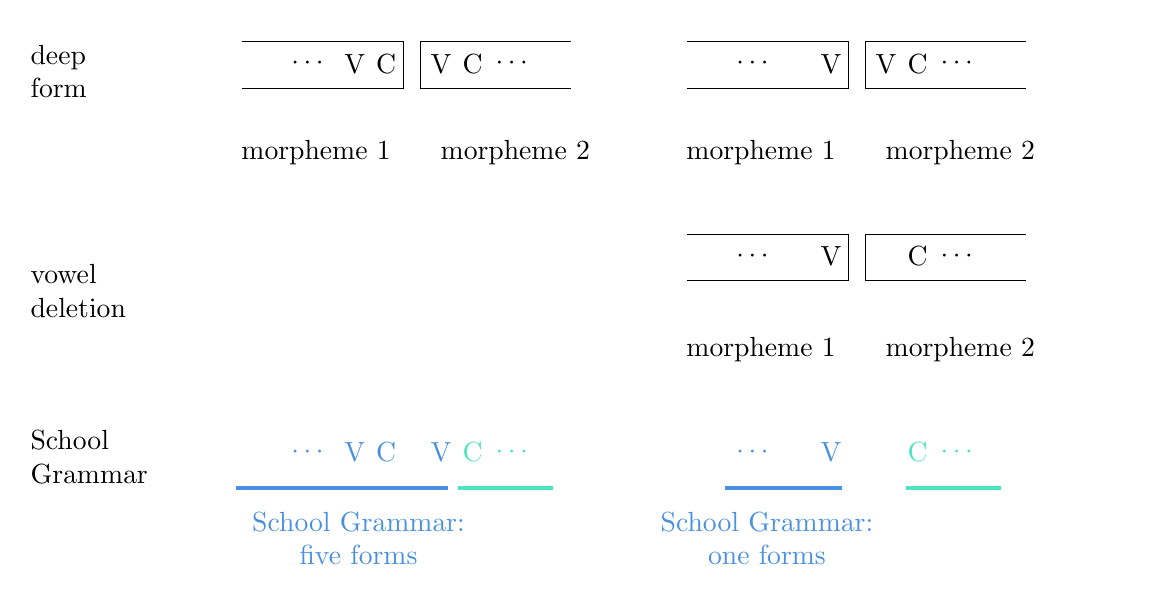
\begin{tikzpicture}[x=0.75pt,y=0.75pt,yscale=-0.8,xscale=0.8]
%uncomment if require: \path (0,419); %set diagram left start at 0, and has height of 419

%Shape: Rectangle [id:dp10799671156840329] 
\draw   (127,59) -- (242,59) -- (242,87.26) -- (127,87.26) -- cycle ;
%Shape: Rectangle [id:dp7035738070234729] 
\draw  [draw opacity=0][fill={rgb, 255:red, 255; green, 255; blue, 255 }  ,fill opacity=1 ] (75,51) -- (145,51) -- (145,101.26) -- (75,101.26) -- cycle ;
%Shape: Rectangle [id:dp9892285153067764] 
\draw   (367,59) -- (252,59) -- (252,87.26) -- (367,87.26) -- cycle ;
%Shape: Rectangle [id:dp10620314732910852] 
\draw  [draw opacity=0][fill={rgb, 255:red, 255; green, 255; blue, 255 }  ,fill opacity=1 ] (419,51) -- (349,51) -- (349,101.26) -- (419,101.26) -- cycle ;
%Straight Lines [id:da8787945793208012] 
\draw [color={rgb, 255:red, 74; green, 144; blue, 226 }  ,draw opacity=1 ][line width=1.5]    (141,328) -- (269,328) ;
%Straight Lines [id:da8747858480961948] 
\draw [color={rgb, 255:red, 80; green, 227; blue, 194 }  ,draw opacity=1 ][line width=1.5]    (275,328) -- (332,328) ;
%Shape: Rectangle [id:dp6953628572273307] 
\draw   (395,59) -- (510,59) -- (510,87.26) -- (395,87.26) -- cycle ;
%Shape: Rectangle [id:dp7297753746089688] 
\draw  [draw opacity=0][fill={rgb, 255:red, 255; green, 255; blue, 255 }  ,fill opacity=1 ] (343,51) -- (413,51) -- (413,101.26) -- (343,101.26) -- cycle ;
%Shape: Rectangle [id:dp6894546413420739] 
\draw   (635,59) -- (520,59) -- (520,87.26) -- (635,87.26) -- cycle ;
%Shape: Rectangle [id:dp45213728860443014] 
\draw  [draw opacity=0][fill={rgb, 255:red, 255; green, 255; blue, 255 }  ,fill opacity=1 ] (687,51) -- (617,51) -- (617,101.26) -- (687,101.26) -- cycle ;
%Shape: Rectangle [id:dp3701432068489623] 
\draw  [draw opacity=0][fill={rgb, 255:red, 255; green, 255; blue, 255 }  ,fill opacity=1 ] (419,167) -- (349,167) -- (349,217.26) -- (419,217.26) -- cycle ;
%Shape: Rectangle [id:dp817155790614746] 
\draw   (395,175) -- (510,175) -- (510,203.26) -- (395,203.26) -- cycle ;
%Shape: Rectangle [id:dp37068543633689766] 
\draw  [draw opacity=0][fill={rgb, 255:red, 255; green, 255; blue, 255 }  ,fill opacity=1 ] (343,167) -- (413,167) -- (413,217.26) -- (343,217.26) -- cycle ;
%Shape: Rectangle [id:dp6500545934497894] 
\draw   (635,175) -- (520,175) -- (520,203.26) -- (635,203.26) -- cycle ;
%Shape: Rectangle [id:dp2082546715911775] 
\draw  [draw opacity=0][fill={rgb, 255:red, 255; green, 255; blue, 255 }  ,fill opacity=1 ] (687,167) -- (617,167) -- (617,217.26) -- (687,217.26) -- cycle ;
%Straight Lines [id:da5254065506928987] 
\draw [color={rgb, 255:red, 74; green, 144; blue, 226 }  ,draw opacity=1 ][line width=1.5]    (436,328) -- (506,328) ;
%Straight Lines [id:da8747110539789369] 
\draw [color={rgb, 255:red, 80; green, 227; blue, 194 }  ,draw opacity=1 ][line width=1.5]    (545,328) -- (602,328) ;

% Text Node
\draw (205,72.5) node [anchor=west] [inner sep=0.75pt]   [align=left] {V};
% Text Node
\draw (224.17,72.5) node [anchor=west] [inner sep=0.75pt]   [align=left] {C};
% Text Node
\draw (173,72.33) node [anchor=west] [inner sep=0.75pt]   [align=left] {$\displaystyle \cdots $};
% Text Node
\draw (257,72.5) node [anchor=west] [inner sep=0.75pt]   [align=left] {V};
% Text Node
\draw (276.17,72.5) node [anchor=west] [inner sep=0.75pt]   [align=left] {C};
% Text Node
\draw (296,72.33) node [anchor=west] [inner sep=0.75pt]   [align=left] {$\displaystyle \cdots $};
% Text Node
\draw (143,117) node [anchor=north west][inner sep=0.75pt]   [align=left] {morpheme 1};
% Text Node
\draw (263,117) node [anchor=north west][inner sep=0.75pt]   [align=left] {morpheme 2};
% Text Node
\draw (205,306.5) node [anchor=west] [inner sep=0.75pt]  [color={rgb, 255:red, 74; green, 144; blue, 226 }  ,opacity=1 ] [align=left] {V};
% Text Node
\draw (224.17,306.5) node [anchor=west] [inner sep=0.75pt]  [color={rgb, 255:red, 74; green, 144; blue, 226 }  ,opacity=1 ] [align=left] {C};
% Text Node
\draw (173,306.33) node [anchor=west] [inner sep=0.75pt]  [color={rgb, 255:red, 74; green, 144; blue, 226 }  ,opacity=1 ] [align=left] {$\displaystyle \cdots $};
% Text Node
\draw (257,306.5) node [anchor=west] [inner sep=0.75pt]  [color={rgb, 255:red, 74; green, 144; blue, 226 }  ,opacity=1 ] [align=left] {V};
% Text Node
\draw (276.17,306.5) node [anchor=west] [inner sep=0.75pt]  [color={rgb, 255:red, 80; green, 227; blue, 194 }  ,opacity=1 ] [align=left] {C};
% Text Node
\draw (296,306.33) node [anchor=west] [inner sep=0.75pt]  [color={rgb, 255:red, 80; green, 227; blue, 194 }  ,opacity=1 ] [align=left] {$\displaystyle \cdots $};
% Text Node
\draw (16,60) node [anchor=north west][inner sep=0.75pt]   [align=left] {deep\\form};
% Text Node
\draw (16,292) node [anchor=north west][inner sep=0.75pt]   [align=left] {School\\Grammar};
% Text Node
\draw (491.75,72.5) node [anchor=west] [inner sep=0.75pt]   [align=left] {V};
% Text Node
\draw (441,72.33) node [anchor=west] [inner sep=0.75pt]   [align=left] {$\displaystyle \cdots $};
% Text Node
\draw (525,72.5) node [anchor=west] [inner sep=0.75pt]   [align=left] {V};
% Text Node
\draw (544.17,72.5) node [anchor=west] [inner sep=0.75pt]   [align=left] {C};
% Text Node
\draw (564,72.33) node [anchor=west] [inner sep=0.75pt]   [align=left] {$\displaystyle \cdots $};
% Text Node
\draw (411,117) node [anchor=north west][inner sep=0.75pt]   [align=left] {morpheme 1};
% Text Node
\draw (531,117) node [anchor=north west][inner sep=0.75pt]   [align=left] {morpheme 2};
% Text Node
\draw (16,192) node [anchor=north west][inner sep=0.75pt]   [align=left] {vowel \\deletion};
% Text Node
\draw (491.75,188.5) node [anchor=west] [inner sep=0.75pt]   [align=left] {V};
% Text Node
\draw (441,188.33) node [anchor=west] [inner sep=0.75pt]   [align=left] {$\displaystyle \cdots $};
% Text Node
\draw (544.17,188.5) node [anchor=west] [inner sep=0.75pt]   [align=left] {C};
% Text Node
\draw (564,188.33) node [anchor=west] [inner sep=0.75pt]   [align=left] {$\displaystyle \cdots $};
% Text Node
\draw (411,236) node [anchor=north west][inner sep=0.75pt]   [align=left] {morpheme 1};
% Text Node
\draw (531,236) node [anchor=north west][inner sep=0.75pt]   [align=left] {morpheme 2};
% Text Node
\draw (491.75,306.5) node [anchor=west] [inner sep=0.75pt]  [color={rgb, 255:red, 74; green, 144; blue, 226 }  ,opacity=1 ] [align=left] {V};
% Text Node
\draw (441,306.33) node [anchor=west] [inner sep=0.75pt]  [color={rgb, 255:red, 74; green, 144; blue, 226 }  ,opacity=1 ] [align=left] {$\displaystyle \cdots $};
% Text Node
\draw (544.17,306.5) node [anchor=west] [inner sep=0.75pt]  [color={rgb, 255:red, 80; green, 227; blue, 194 }  ,opacity=1 ] [align=left] {C};
% Text Node
\draw (564,306.33) node [anchor=west] [inner sep=0.75pt]  [color={rgb, 255:red, 80; green, 227; blue, 194 }  ,opacity=1 ] [align=left] {$\displaystyle \cdots $};
% Text Node
\draw (146,341) node [anchor=north west][inner sep=0.75pt]  [color={rgb, 255:red, 74; green, 144; blue, 226 }  ,opacity=1 ] [align=left] {\begin{minipage}[lt]{80.99pt}\setlength\topsep{0pt}
\begin{center}
School Grammar:\\five forms
\end{center}

\end{minipage}};
% Text Node
\draw (392,341) node [anchor=north west][inner sep=0.75pt]  [color={rgb, 255:red, 74; green, 144; blue, 226 }  ,opacity=1 ] [align=left] {\begin{minipage}[lt]{80.99pt}\setlength\topsep{0pt}
\begin{center}
School Grammar:\\one forms
\end{center}

\end{minipage}};


\end{tikzpicture}
